\documentclass[notitlepage, reprint, nofootinbib]{revtex4-1}
\usepackage[utf8]{inputenc}

% Mathematics and symbols:
\usepackage{amsmath, gensymb, amsthm, physics, mhchem, amssymb}
% Algorithms: 
\usepackage{algorithm}
\usepackage{algpseudocode}
% Figures:
\usepackage{tikz, graphicx}
\usepackage[caption=false]{subfig}

% Other:
\usepackage{hyperref}


% Document formatting 
\setlength{\parskip}{1mm}
\setlength{\parindent}{0mm}

% Programming
\definecolor{codebackground}{rgb}{0.9,0.9,0.9}
\usepackage{listings}
\lstset{
	language=python,
	backgroundcolor=\color{codebackground},
	basicstyle=\scriptsize,
	aboveskip={1\baselineskip},
	columns=fixed,
	numbers=left,
	showstringspaces=false, 
	breaklines=true,  
	frame=single,
	showtabs=false,
	showspaces=false,
	keywordstyle=\color[rgb]{0,0,1},
	commentstyle=\color[rgb]{0.133,0.545,0.133}
	}

\hypersetup{
    colorlinks=true,
    citecolor=violet,
    linkcolor=orange,
    filecolor=orange,      
    urlcolor=orange,
}

\begin{document}
\title{FYS-STK4155 - Project 2}
\author{Frida Larsen}

\begin{abstract}
The aim of this project was to compare Ridge and logistic regression with neural networks in terms of limitations and benefits. Four analyses were performed on two data sets: two for regression using data based on the Franke function and two for classification using the MNIST data set. We found that the neural networks could produce results of the same quality as the more traditional methods, but that they proved more difficult to set up and optimise. The results produced by the neural networks were also harder to interpret, especially for the more complex architectures implemented.
\end{abstract}

\maketitle

\section{Introduction}
Ridge and logistic regression are two methods that have been extensively used in prediction analysis. In recent years, neural networks have become increasingly popular as a tool for both regression and classification analysis. The strength of neural networks lie in their more complex architecture, but comes at a cost of loss of interpretability.\\[2mm]
The overarching aim of this project is to compare Ridge and logistic regression with neural networks. Are the neural networks able to achieve better results and under what constraints? What are the benefits and limitations of the different approaches? \\[2mm]
We will use two data sets to compare and quantify our models. For the regression methods we will use a data set based on the Franke function. For the classification methods we will use the well-known MNIST data set. \\[2mm]
We will begin with a description of the methods and data sets before moving on to describing the procedures of the experiments. All relevant code may be found in the GitHub repository 'FYS-STK4155'\footnote{\href{GitHub Repository}{https://github.com/fridalarsen/FYS-STK4155}} under the Project2 folder. This folder also includes a Figures folder, which holds all the figures presented in this text and produced during the project.

\section{Methods}
The methods and theory presented in this section are based on the lecture notes from Morten Hjorth-Jensen \cite{lecturenotes3}\cite{lecturenotes1}\cite{lecturenotes2}, Hastie et al's book \emph{The Elements of Statistical Learning} \cite{ESL} and Nielsen's book \emph{Neural Networks and Deep Learning} \cite{nielsen}.\\[2mm]
In general, the regression methods are analysed using the MSE and R$^2$ metrics, whilst the classification methods are analysed using the accuracy metric.

\subsection{Stochastic Gradient Descent}
Many numerical methods are based on determining the parameters that minimise some function, typically denoted as the cost function $C$. The minimum can be found analytically by setting the derivative equal to 0. However, it is not given that the resulting equation is analytically solveable. We therefore need a method for numerically approximating this minimum. \\[2mm]
The main idea of the gradient descent method is to start with some randomly chosen function value, calculate the gradient of the function at this point and take a step in the opposite direction of the gradient (in the direction of which the graph is sinking). The step length is determined by a parameter $\gamma$. Thus we move iteratively towards the lowest point of the function. The iterations go as follows: 
\begin{equation}\label{gd}\vb{a}_{n+1}=\vb{a}_n-\gamma_n\grad F(\vb{a}_n)\end{equation}
where $\grad F$ is the gradient of the cost function. An issue with the standard gradient descent method is that we don't know if the located minimum is global or local, so it is sensitive to initial conditions. This can be solved to a degree by performing a grid search to determine the optimal initial parameters. It is also worth noting that the standard gradient descent method is computationally expensive. \\[2mm]
The stochastic gradient descent (SGD) method aims to solve some of the issues with the standard gradient descent method. SGD is based on the observation that the cost function (in most cases) can be written as a sum over $n$ data points, which means that the gradient can be written as sum over $i$ gradients: 
$$\grad_\beta F(\beta)=\sum_i^n \grad_\beta f_i(\vb{x}_i, \beta).$$
With this in mind, we introduce the stochasticity which gives the SGD method its name: We only compute the gradient based on a subset of the datapoints. Such a subset is called a minibatch. Thus we can replace the sum over the number of points with a sum over the number of points in a minibatch. Implementing all this results in a gradient step given by 
\begin{equation}\label{sgd}\beta_{j+1}=\beta_j-\gamma_j\frac{1}{n}\sum_{i\in B_k}^{n}\grad_\beta f_i(\vb{x}_i, \beta_j)\end{equation}
where M is the size of each minibatch, Bk is the kth minibatch, gamma is the learning parameter and n/M is the number of minibatches. One iteration over the number of minibatches is called an epoch. 

\subsection{Ridge regression}
Ridge regression is a regression method for predicting a continuous output $\vb{z}$ based on input observations $X$. The predictions are given by 
\begin{equation} \vb{z}=X\boldsymbol{\beta},\end{equation} 
where $\boldsymbol{\beta}$ is a vector of regression coefficients. The Ridge regression method aims to find the $\beta$ coefficients that minimise the mean squared error (MSE) of the prediction, subject to an L$^2$-penalty described by the parameter $\lambda$. Including a non-zero penalty forces the size of the coefficients to decrease when compared to the non-penalised case. The cost function is 
\begin{align}
	C(X,\boldsymbol{\beta})&=MSE+L^2\text{-penalty}\\
	&=(\vb{y}-X\boldsymbol{\beta})^T(\vb{y}-X\boldsymbol{\beta})+\lambda\boldsymbol{\beta}^T\boldsymbol{\beta}.
\end{align}
In the case of Ridge regression there is an analytical solution to the minimisation problem. In order to find an expression for the minimum of C, we will need the derivative:
$$\pdv{C}{\boldsymbol{\beta}}=-\frac{1}{n}2X^T(\vb{z}-X\boldsymbol{\beta})+2\lambda\boldsymbol{\beta}$$
C will reach is minimum when this is 0:
$$-\frac{1}{n}2X^T(\vb{z}-X\boldsymbol{\beta})+2\lambda\boldsymbol{\beta}=0.$$
From this we get
\begin{align*}
	&\frac{1}{n}X^T\vb{z}=(\frac{1}{n}X^TX+\lambda I)\boldsymbol{\beta}\\
	&\Rightarrow \boldsymbol{\beta}=\frac{1}{n}(\frac{1}{n}X^TX+\lambda I)^{-1}X^T\vb{z}\\
	&\quad\quad\  =(X^TX+n\lambda I)^{-1}X^T\vb{z}
\end{align*}
We rename $n\lambda$ as simply $\lambda$ and end up with 
\begin{equation}\label{ridge}\boldsymbol{\beta}=(X^TX+\lambda I)^{-1}X^T\vb{y}.\end{equation}
Note that $\lambda=0$ is equivalent to the ordinary least squares (OLS) method. \\[2mm]
Equation \ref{ridge} gives us an analytical way of determining the $\boldsymbol{\beta}$ that minimises the cost function. However, this can also be estimated numerically through the SGD method.

\subsection{Logistic regression}
Logistic regression is a method for classification, meaning that the method can be used for predicting a discrete output $\vb{z}$ based on input observations $X$. For a given problem with $K$ classes, the method works by assigning probabilities to each class using the softmax function: 
\begin{equation}p_i=\sigma(\vb{z})_i = \frac{e^{z_i}}{\sum_{j=1}^K e{z_j}},\end{equation}
where $\vb{z}=X\boldsymbol{\beta}$, and $\boldsymbol{\beta}$ are regression coefficients similar to those of Ridge regression. The final classification of an input is then given by the class with the greatest probability. \\[2mm]
The mean squared error does not take the probabilistic nature of the predictions into account. We therefore wish to use a different cost function for logistic regression. The main idea is to maximise the likelihood of predicting the correct classes. For a given observation in class $k\in \{1,2,\dots, K\}$ we let $t_i^k$ be 1 if $i=k$ and 0 otherwise. The likelihood can then be written as 
\begin{equation}\mathcal{L}(\boldsymbol{\beta}|\vb{z},k)=\prod_{i=1}^K z_i^{t_i^k}\end{equation}
Maximising the likelihood is equivalent to minimising the negative log-likelihood, which we will take as our cost function. By expanding the log and adding the contributions from each observation $n$ we get   
\begin{equation}C(X, \boldsymbol{\beta})=-\sum_{n=1}^N \sum_{i=1}^K t_i^{k_n}  \log (z_i)\end{equation}
In addition, we will regularise the regression coefficients using a similar penalty term as in Ridge regression. As there is no analytical solution to this minimisation problem, we must resort to numerical methods. We will use SGD.  

\subsection{Neural networks}
A neural network is a data structure or algorithm inspired by how the neurons in the brain are organised. \cite{snl_NN} Due to their complex structure, neural networks are capable of performing a large variety of tasks, both regression and classification problems. As for logistic regression, there is no analytical solution to the minimisation of the cost functions, so we will use the SGD algorithm we have developed in order to solve our minimisation problems. Computing the derivative of the cost function is more difficult for neural networks than for Ridge and logistic regression. This is where the back propagation algorithm comes in. Before developing this algorithm, we must explore the structure of the network.   

\subsubsection{Feed forward}
One of the main subspecies of neural networks is the basic artificial neural network (ANN), which consists of "neurons" (called nodes) collected in layers. The first layer is called the input layer and the last layer is called the output layer. The layers in between are known as hidden layers. Information can pass between nodes of different layers and each connection between nodes is associated with a weight. \\[2mm]
A feed forward neural network (FFNN) is a type of ANN. An FFNN is structured so that information is only able to flow in one direction: forward through the layers. In addition, the network is fully connected, so that each node in a layer is connected to all the nodes in the next layer. An FFNN with more than three layers is known as a multilayered perceptron (MLP). In our implementation we have chosen to use the same number of nodes in each hidden layer. \\[2mm]
The information sent from one layer to the next is represented by  
\begin{equation} y_i^l=f^l(z_i^l)=f^l\Big(\sum_{j=1}^{N_{l-1}}w_{ij}^l y_j^{l-1}+b_i^l \Big).\end{equation}
Here, $w_{ij}^{l}$ is the weight connecting node $i$ in layer $l-1$ to node $j$ in layer $l$. $b_i^l$ are additional bias terms added for normalisation. The function $f^l$ is known as the activation function of layer $l$, which is non-linear. In principle, each activation function can be different for each hidden layer, but we have opted to use the same activation function for each layer. In particular, we will use the tanh activation function. Similar attempts were made with the sigmoid function, but the results turned out superior with the tanh function.  

\subsubsection{Back propagation}
In order to use stochastic gradient descent for minimising our cost function, we need the gradient of our cost function with respect to the weights and biases (the parameters for which we want to minimise the cost function). \\[2mm]
The error of node j in layer l is defined by \cite[chpt 2]{nielsen} 
\begin{equation}\label{error}\delta_j^l=\pdv{C}{z_j^l}\end{equation}
Note that with this definition we have that
\begin{equation}\label{bp3}\delta_j^l = \pdv{C}{b_j^l},\end{equation}
since
$$ \pdv{C}{b_j^l}=\pdv{C}{z_j^l}\pdv{z_j^l}{b_j^l}=\pdv{C}{z_j^l}.$$
The error of the output layer (layer L) is given by 
\begin{equation}\label{output_error}\delta_j^L=f'(z_j^L)\pdv{C}{a_j^L}.\end{equation}
The error of any layer can be found in terms of the error of the next layer by 
\begin{equation}\label{bp2}\delta_j^l=\sum_k \delta_k^{l+1}w_{kj}^{l+1}f'(z_j^l).\end{equation}
This is known as back propagating the error as it calculated the error in layer $l$ using the error in layer $l+1$. The derivative of the cost function with respect to the weights are given by
\begin{equation}\label{bp4}\pdv{C}{w_{jk}^L}=\delta_j^L a_k^{L-1}.\end{equation}
By combining these equations we get the back propagation algorithm for determining the gradient of C: 
\begin{algorithm}[H]
	\caption{Back propagation}
	\begin{algorithmic}[1]
		\State Compute error in output layer, $\delta_j^L$, via equation \ref{output_error}.
		\State Compute error of each layer backwards from the output via equation \ref{bp2}.
		\State Compute the derivative of C with respect to biases and weights from equations \ref{bp3} and \ref{bp4} respectively.
	\end{algorithmic}
\end{algorithm}
The gradient of C is then fed to the stochastic gradient descent algorithm, which updates the weights and biases. 



\begin{figure}[h!]
	\centering
	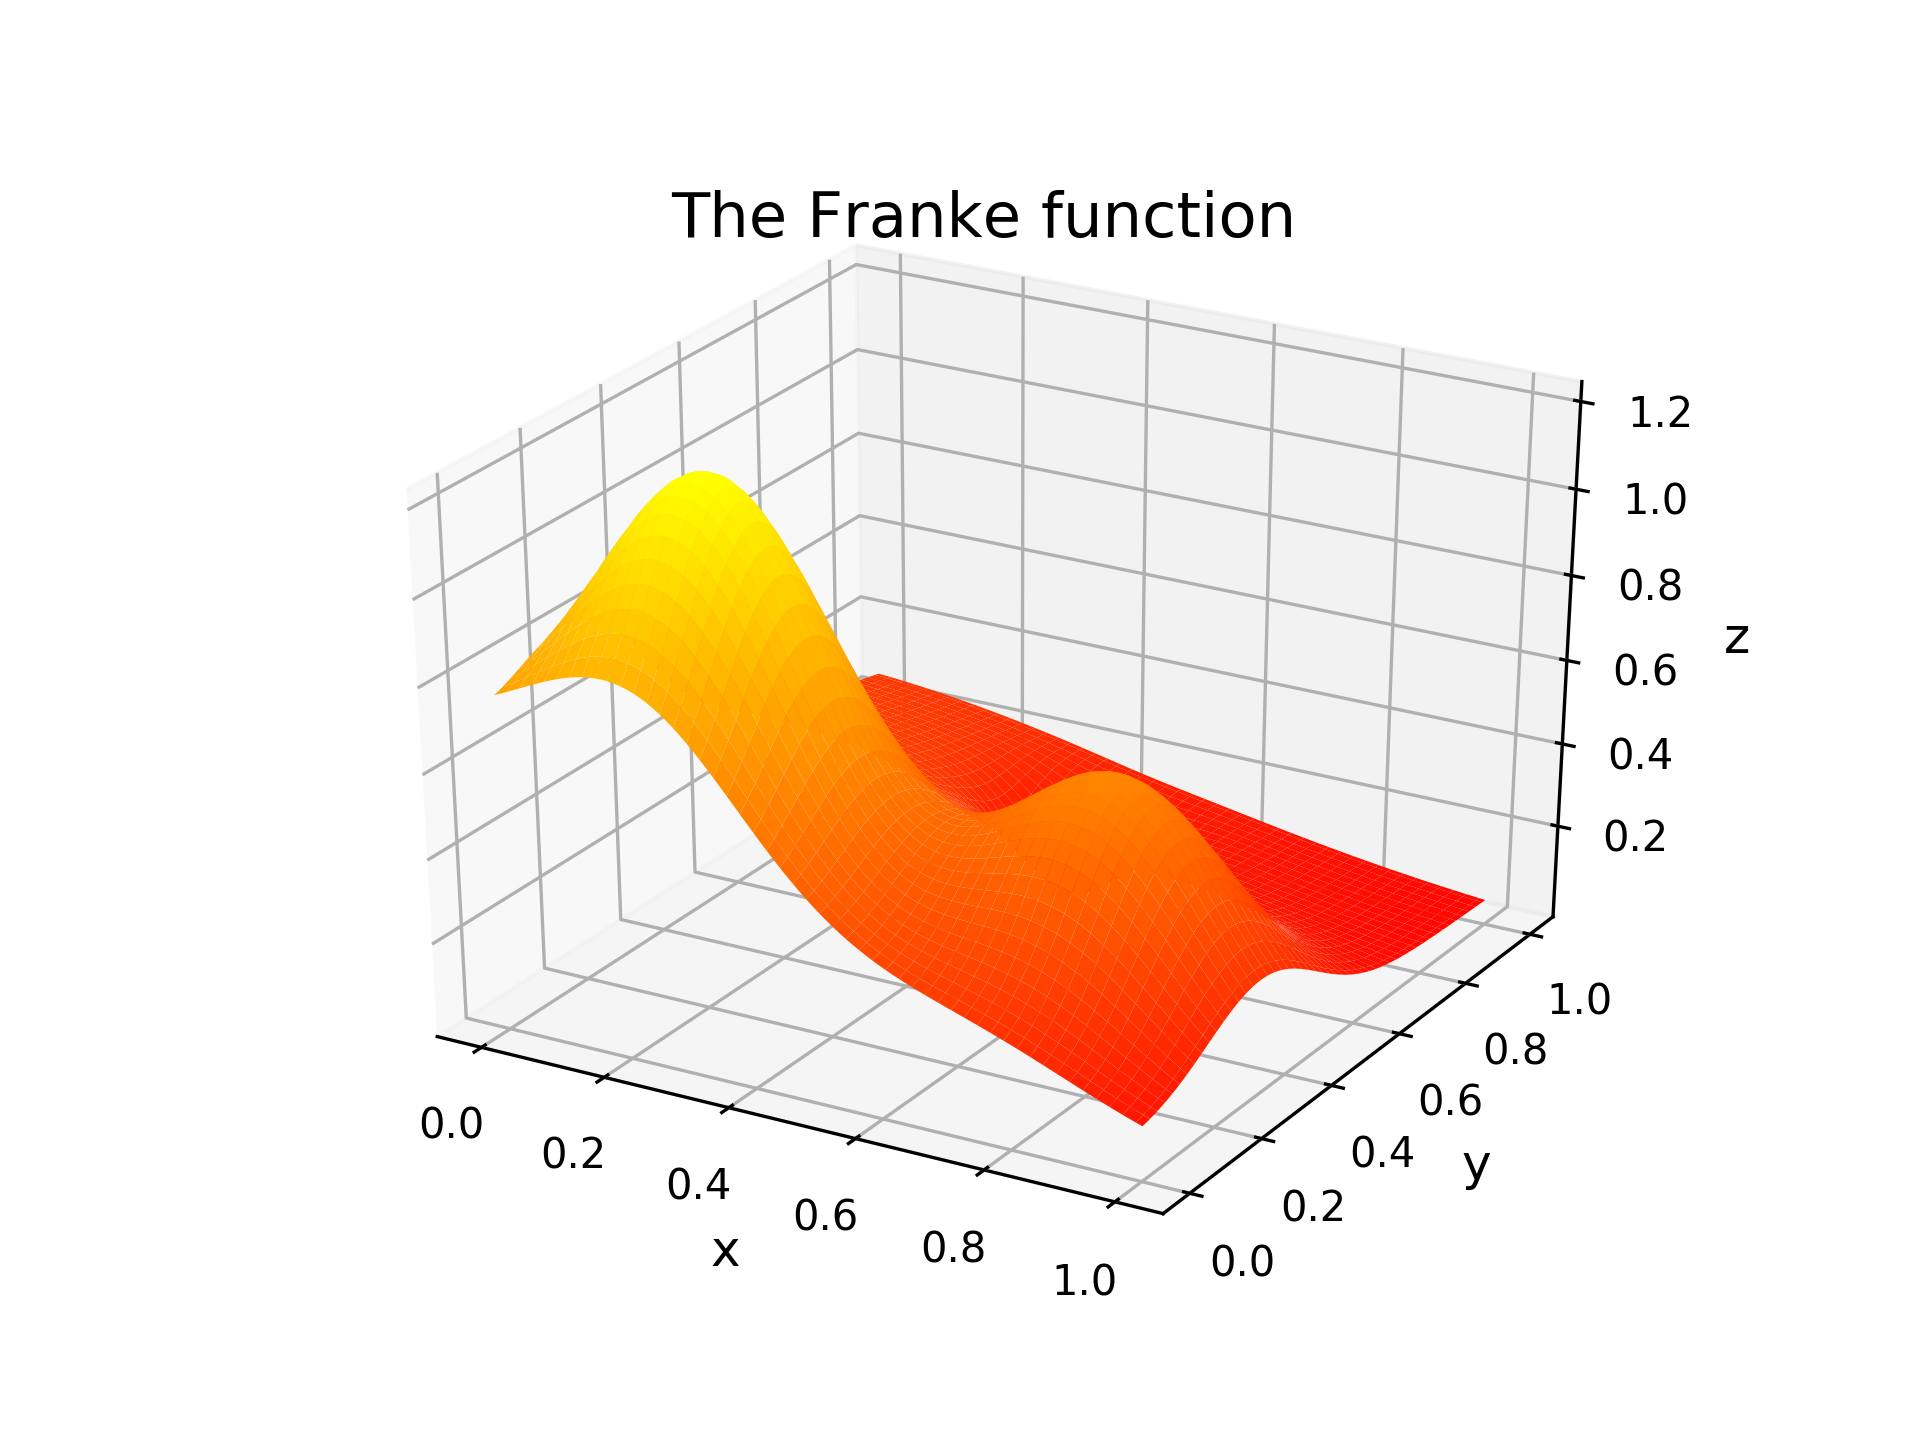
\includegraphics[width=0.45\textwidth]{../Figures/franke_function.png}
	\caption{The Franke function.}
	\label{franke}
\end{figure}
\subsection{Data sets}
\subsubsection{The Franke function}
The function we will use to investigate our regression methods is known as the Franke function. It is given by 
\begin{align}
	f(x,y)=&\frac{3}{4}\exp\Big(-\frac{(9x-2)^2}{4}-\frac{(9y-2)^2}{4}\Big)\nonumber\\
	&+\frac{3}{4}\exp\Big(-\frac{(9x+1)^2}{49}-\frac{(9y+1}{10}\Big)\nonumber\\
	&+\frac{1}{2}\exp\Big(-\frac{(9x-7)^2}{4}-\frac{(9y-3)^2}{4}\Big)\nonumber\\
	&-\frac{1}{5}\exp\Big(-(9x-4)^2-(9y-7)^2\Big)
\end{align} 
The function is plotted in figure \ref{franke}. We will use $x$- and $y$-values in the range $[0,1]$, and add a normally distributed error to $f(x,y)$ with standard deviation $\sigma=0.1$.

\subsubsection{The MNIST dataset}
The MNIST dataset is a large dataset containing images of handwritten numbers with labels containing their digits (0-9). The \texttt{sklearn} dataset \texttt{digits}\footnote{The dataset is described in detail at \url{https://scikit-learn.org/stable/datasets/index.html\#digits-dataset}} contains a selection of the MNIST data, and is the data set that we will use for the classification part of this report. \\[2mm]
Figure \ref{MNIST_example} shows an example of one of the MNIST images. 
\begin{figure}
	\centering
	\includegraphics[width=0.45\textwidth]{../Figures/MNIST_example.png}
	\caption{An image from the MNIST dataset showing the number 8. }
	\label{MNIST_example}
\end{figure}

\subsection{Procedures}
\subsubsection{Evaluating the SGD algorithm}
In order to evaluate the SGD algorithm we will compare Ridge regression using SGD to approximate the optimal $\boldsymbol{\beta}$ and normal Ridge regression using matrix inversion to find the optimal $\boldsymbol{\beta}$ via equation \ref{ridge}. By comparing the coefficient estimates of the SGD method to the analytical values, we can determine whether the algorithm is successful in solving the minimisation problem. We can also use this comparison to determine the best parameters for the SGD-based Ridge regression.  This comparison will serve as an indicator for the algorithm's performance and accuracy with regards to logistic regression and neural networks. \\[2mm]
First, we will investigate whether the SGD Ridge regression is able to converge to a solution at all, and how many epochs are required for it do so. We will use a variety of penalties and sufficient learning parameters. Second, we will perform a grid search in order to determine the best learning parameters. Lastly, we will investigate the impact of the number of minibatches on the cost function.

\subsubsection{Neural network regression}
For regression using a neural network our goal is to determine the best parameters for our model. The first step is to determine the effect of penalties on the evolution of the cost function. \\[2mm]
Secondly, we want to determine the best learning parameters for our model. This will be done with a grid search using the cost function to determine the best parameters. \\[2mm]
Next, we will investigate the effect of the neural network architecture. In particular, we will study the mean squared error and the R$^2$-score for several numbers of nodes and layers. \\[2mm]
Lastly, we will use three representative architectures and study the effect of different penalties in these cases in terms of mean squared error and R$^2$-scores. . 

\newpage
\subsubsection{Logistic regression}
Firstly, we will investigate the convergence of the cost function for a selection of penalties as a function of epochs. \\[2mm]
We then wish to determine the optimal learning parameters. This will be done by performing a grid search with the learning parameters and how they affect the cost function. The next step is to study the effect of the penalty parameter on our model. We will run the simulation for different penalties and calculate the accuracy score in order to determine which penalty is the optimal one. 

\subsubsection{Neural network classification}
We begin by investigating the evolution of the cost function for a variety of penalties as a function of the number of epochs. \\[2mm]
In order to determine the optimal learning parameters we will perform a grid search and determining what parameters minimise the cost function. \\[2mm]
In order to determine the best architecture, a grid search based on the accuracy score for a variety of number of nodes and layers will be performed. For three chosen architectures, the accuracies are studied for different penalties. 

\section{Results}
\subsection{Evaluating the SGD algorithm}
Figure \ref{fig1} shows the evolution of the Ridge regression cost function for four different penalties during 1000 epochs. Figure \ref{fig2} shows the difference in coefficient estimates as produced by Ridge regression with SGD and matrix inversion for a variety of learning parameters. A similar plot is shown in figure \ref{fig3}, however here we show the Ridge cost function instead of the difference in coefficient estimates. Figure \ref{fig4} shows the evolution of the cost function for different sized minibatches. 

\begin{figure}
	\centering 
	\includegraphics[width=0.45\textwidth]{../Figures/ridge_sgd_cost_function.png}
	\caption{Evolution of the Ridge regression cost function during 1000 epochs for four different penalty parameters.}
	\label{fig1}
\end{figure}

\begin{figure}
	\centering 
	\includegraphics[width=0.45\textwidth]{../Figures/ridge_sgd_beta_diff.png}
	\caption{Difference in regression coefficient estimates for Ridge regression using matrix inversion and SGD for different learning parameters.}
	\label{fig2}
\end{figure}

\begin{figure}
	\centering 
	\includegraphics[width=0.45\textwidth]{../Figures/ridge_sgd_C.png}
	\caption{Difference in cost function for Ridge regression using matrix inversion and SGD for different learning parameters.}
	\label{fig3}
\end{figure}

\begin{figure}
	\centering 
	\includegraphics[width=0.45\textwidth]{../Figures/ridge_sgd_cost_function2.png}
	\caption{Evolution of the cost function in Ridge regression using SGD for different number of minibatches $n$. }
	\label{fig4}
\end{figure}

\subsection{Neural network regression}
Figure \ref{fig5} shows the evolution of the cost function of the neural network for different penalties during 200 epochs. The zero penalty case is shown in figure \ref{fig6} for a variety of learning parameters. Figures \ref{fig7} and \ref{fig8} show the MSE and the R$^2$ score for various architectures. Figures \ref{fig9} and \ref{fig10} show the MSE and R$^2$-scores for a range of different penalties for three different architectures. 

\begin{figure}
	\centering 
	\includegraphics[width=0.45\textwidth]{../Figures/NN_sgd_cost_function.png}
	\caption{Evolution of the neural network regression cost function for different penalties.}
	\label{fig5}
\end{figure}

\begin{figure}
	\centering 
	\includegraphics[width=0.45\textwidth]{../Figures/NNreg_learning_params_log.png}
	\caption{Value of neural network regression cost function for a variety of learning parameters. The white areas indicate a diverging result. }
	\label{fig6}
\end{figure}

\begin{figure}
	\centering 
	\includegraphics[width=0.45\textwidth]{../Figures/NNreg_MSE_architecture.png}
	\caption{Mean squared error of the neural network regression for various numbers of nodes and layers. }
	\label{fig7}
\end{figure}

\begin{figure}
	\centering 
	\includegraphics[width=0.45\textwidth]{../Figures/NNreg_R2_architecture.png}
	\caption{R$^2$-score of the neural network regression for various numbers of nodes and layers. }
	\label{fig8}
\end{figure}

\begin{figure}
	\centering 
	\includegraphics[width=0.45\textwidth]{../Figures/NNreg_MSE_penalties.png}
	\caption{The mean squared error for a range of penalties, shown for three different architectures.}
	\label{fig9}
\end{figure}

\begin{figure}
	\centering 
	\includegraphics[width=0.45\textwidth]{../Figures/NNreg_R2_penalties.png}
	\caption{The R$^2$-score for a range of penalties, shown for three different architectures.}
	\label{fig10}
\end{figure}

\subsection{Logistic regression}
Figure \ref{fig11} shows the evolution of the logistic regression cost function for different penalties during 200 epochs. Figure \ref{fig12} shows the cost function for a range of learning parameters for the 0 penalty case. Figure \ref{fig13} shows the accuracy score for a range of penalties.

\begin{figure}
	\centering 
	\includegraphics[width=0.45\textwidth]{../Figures/LR_sgd_cost_function.png}
	\caption{Evolution of logistic regression cost function for different penalties.}
	\label{fig11}
\end{figure}

\begin{figure}
	\centering 
	\includegraphics[width=0.45\textwidth]{../Figures/LR_learning_params_lin.png}
	\caption{The logistic regression cost function for ranges of the two learning parameters.}
	\label{fig12}
\end{figure}

\begin{figure}
	\centering 
	\includegraphics[width=0.45\textwidth]{../Figures/LRreg_acc_penalties.png}
	\caption{Accuracy of the logistic regression model for a range of penalties.}
	\label{fig13}
\end{figure}

\subsection{Neural network classification}
Figure \ref{fig14} shows the evolution of the cost function of the neural network for different penalties during 200 epochs. The zero penalty case is shown in figure \ref{fig15} for a range of learning parameters. Figures \ref{fig16} and \ref{fig17} show the accuracy of the classification for different architectures and penalties respectively.


\begin{figure}
	\centering 
	\includegraphics[width=0.45\textwidth]{../Figures/NNcla_sgd_cost_function.png}
	\caption{Evolution of the neural network classification cost function for different penalties.}
	\label{fig14}
\end{figure}

\begin{figure}
	\centering 
	\includegraphics[width=0.45\textwidth]{../Figures/NNcla_learning_params_lin.png}
	\caption{The neural network classification cost function for a range of learning parameters.}
	\label{fig15}
\end{figure}

\begin{figure}
	\centering 
	\includegraphics[width=0.45\textwidth]{../Figures/NNcla_acc_architecture2.png}
	\caption{Accuracy score for classification neural network with a range of architectures. }
	\label{fig16}
\end{figure}

\begin{figure}
	\centering 
	\includegraphics[width=0.45\textwidth]{../Figures/NNcla_acc_penalties.png}
	\caption{Accuracy score for classification neural network for a range of penalties.}
	\label{fig17}
\end{figure}


\section{Discussion}
Overall, the neural networks score well in terms of MSE for regression and accuracy for classification when compared to Ridge and logistic regression. However, finding the optimal architectures are often computationally heavy tasks. Furthermore, algorithms trained with SGD were surprisingly sensitive to the learning scheme and the learning parameters chosen. \\[2mm]
For the Ridge experiment, figure \ref{fig1} shows that the cost function has an initial phase of quick convergence before moving to a fine tuning phase as the learning rate decreases and the gradient is closer to 0. However, as seen from figures \ref{fig2} and \ref{fig3}, there are some combinations of learning parameters that give better results than others. Convergence is achieved for a large span of learning parameters. In addition, figure \ref{fig4} shows that the number of minibatches has little impact on the overall performance of the model. \\[2mm]
For the neural network regression, figure \ref{fig5} shows that the cost function converges quickly, similar to the Ridge regression case. Unlike Ridge regression, the fine tuning phase is less relevant as the cost function is fairly stable after the initial drop. Another important difference is that the neural network regression proved to be very sensitive to the learning parameters chosen. Specifically, some combinations lead to a divergence of the cost function as seen in figure \ref{fig6}. Notably, the optimal learning parameters are close to the boundary of convergent combinations. These specific parameters correspond to fast learning. So we see that fast learning may provide a good model, but is susceptible to diverging. \\[2mm]
When it comes to the network architecture, we see from figure \ref{fig7} that the more complex regression networks perform better. However, since the difference is relatively small it is worth asking whether this decrease in mean squared error is worth it when the model is so complex that we cannot interpret it properly.  \\[2mm]
For the logistic regression experiment, figure \ref{fig11} shows that the cost function is quick to converge for all penalties. Interestingly, the curve with the highest penalty converges to a much lower level than the other curves. This is particularly interesting, because adding a higher penalty typically leads to a larger cost functions, as we have seen in the other experiments. From figure \ref{fig13} we see that the optimal penalty is around 2. Overall, the logistic regression is very stable.\\[2mm]
For the neural network classification we see from figure \ref{fig14} that the cost function converges. However, the shape of the curves are very different to the corresponding curves for the other experiments. We observe that the cost function evolves in bursts as a consequence of the uneven shape of the cost function (it is not convex and has plenty of local minima). When it comes to the learning parameters of figure \ref{fig15} we see that there is a clear region of optimisation. \\[2mm]
Interestingly, we find from figure \ref{fig16} that a more complex architecture is not preferred in the classification case in the no penalty case. Figure \ref{fig17} seems to suggest the opposite for a penalised network, but we see that the architecture chosen in this case is on the boundary of the area where we expect a higher accuracy. 
\section{Conclusion}
Our aim was to compare Ridge and logistic regression with neural networks in terms of benefits and limitations. We found that Ridge and logistic regression can be trained with a large variety of learning parameters and provide reasonable results for most penalties. Additionally, they only require fine tuning of the penalty parameter. In contrast, the neural networks required more computationally heavy fitting due to their higher level of complexity. Optimal results were only achievable for a subset of the learning parameters and architectures, which provides an additional computational barrier. \\[2mm]
Future studies should look into the effect of different learning schemes and gradient descent method with the aim of finding a more stable network. 

\bibliographystyle{unsrtnat}
\bibliography{references.bib}



\end{document}